\section{Lifetime}

Every variable is \textit{\textbf{created}} (or \textit{allocated}) at some definite time, and \textit{\textbf{destroyed}} (or \textit{deallocated}) at some later time when it is no longer needed. \textit{The interval between creation and destruction} of a variable is called its \textit{\textbf{lifetime}}.

The concept of lifetime is pragmatically important. A variable needs to occupy storage cells only during its lifetime. We can classify variables according to their lifetimes:
\begin{itemize}
  \item A \textit{\textbf{global variable}}'s lifetime is \textit{the program's run-time}.
  \item A \textit{\textbf{local variable}}'s lifetime is \textit{an activation of a block}.
  \item A \textit{\textbf{heap variable}}'s lifetime is \textit{arbitrary, but is bounded by the program's run-time.}
  \item A \textit{\textbf{persistent variable}}'s lifetime is \textit{arbitrary, and may transcend the run-time of any particular program}.
\end{itemize}

\subsection{Global and Local Variables}

A \textit{\textbf{global variable}} is one that is declared for use throughout the program. A global variable's lifetime is the program's entire run-time: \textit{the variable is created when the program starts, and is destroyed when the program stops}.

A \textit{\textbf{local variable}} is one that is declared within a block, for use only within that block. A lifetime of a local variable is an activation of the block containing that variable's declaration: \textit{the variable is created on entry to the block, and is destroyed on exit from the block.}

A \textit{\textbf{block}} is a program construct that includes local declarations. In all programming languages, the body of a procedure is a block. An \textit{\textbf{activation}} of a block is the time interval during which that block is being executed. In particular, \textit{an activation of a procedure is the time interval between call and return}. During a single run of the program \textit{a block may be activated several times, and so a local variable may have several lifetimes}.

A local variable \textit{cannot retain its content over successive activations of the block} in which it is declared. In some programming languages, a variable may be initialized as part of its declaration. But if a variable is not initialized, its content is \textit{undefined}, \textit{not} the value it might have contained in a previous activation of the block.

Some programming languages (such as \texttt{C}) allow a variable to be declared as a \textit{\textbf{static variable}}, which defines its lifetime to be the program's entire run-time (even if the variable is declared inside a block). Thus static variables have the same lifetime as global variables. Although this feature addresses a genuine need, there are better ways to achieve the same effect, such as class variables in object-oriented languages.

\end{multicols*}

\begin{multicols}{2}
\setlength{\columnsep}{1.5cm}
\setlength{\columnseprule}{0.2pt}

\subsection{Heap Variables}

A \textit{\textbf{heap variable}} is one that can be created, and destroyed, at any time during the program's run-time. A heap variable is created by an expression or command. \textit{It is anonymous, and is accessed through a pointer. (By contrast, a global or local variable is created by a declaration, and has an identifier.)} The lifetimes of heap variables follow no particular pattern. 

Pointers are first-class values, and thus may be stored, used as components of composite values, and so on. 

An \textit{\textbf{allocator}} is an operation that creates a heap variable, yielding a pointer to that heap variable. In \texttt{C++} and \texttt{JAVA}, an expression of the form ``\texttt{\textbf{new}} ...'' is an allocator. (In \texttt{C}, \texttt{malloc()}.)

A \textit{\textbf{deallocator}} is an operation that destroys a given heap variable. \texttt{C++}'s deallocator is a command of the form ``\texttt{\textbf{delete}} ...''. \texttt{JAVA} has no deallocator at all. (In \texttt{C}, \texttt{free()}.) Deallocators are unsafe, since any remaining pointers to a destroyed heap variable become \hyperref[sec:dangling-pointers]{\textit{dangling pointers}}.

A heap variable remains \textit{\textbf{reachable}} as long as it can be accessed by following pointers from a global or local variable. A heap variable's lifetime extends from its creation until it is destroyed or it becomes unreachable.

Sometimes, operating system tolerates dangling references. However, sometimes, it generates run-time erros like ``protection fault'' or ``segmentation fault'' are generated.

\subsubsection{Garbage Variables}

\textit{\textbf{Garbage variables}} are the variables with lifetime still continue but there is no way to access.

\begin{minted}{c}
...
char *p, *q;
p = malloc(10);
p = q;
...
void f() {
  char *p;
  p= malloc(10); ...
  return;
}

f ();
\end{minted}

When the pointer value is lost or lifetime of the pointer is
over, heap variable is unaccessible. (\texttt{*p} in examples)

\subsubsection{Garbage Collection}

A solution to dangling reference and garbage problem is garbage collection. Garbage collection (GC) is a form of automatic memory management. The garbage collector attempts to reclaim memory which was allocated by the program, but is no longer referenced-also called garbage. In other words, PL does management of heap variable deallocation
automatically. \texttt{Java, Lisp, ML, Haskell} and most functional languages provide garbage collection.

Also, Calls like free() or delete does not exist. Language runtime needs to:
\begin{itemize}
  \item Keep a reference counter on each reference, initially 1
  \item Increment counter on each new assignment
  \item Decrement counter at the end of the reference lifetime
  \item Decrement counter at the overwritten/lost references
  \item Do all these operations recursively on composite values.
  \item When reference count gets 0, deallocate the heap variable
\end{itemize}

Garbage collector deallocates heap variables having a reference count 0. Since it may delay execution of tasks, GC is not immediately done. GC usually works in a separate thread, in low priority, works when CPU is idle.

Another but too restrictive solution to garbage is that \textit{reference cannot be assigned to a longer lifetime variable}. Local variable references cannot be assigned to global reference/pointer.

\subsection{Persistent Variables}

\textit{\textbf{Files}} may be seen as composite variables. In particular, a \textit{\textbf{sequential file}} is a sequence of components, and a direct file is (in effect) an array of components.

Usually files contain large bodies of long-lived data: they are \textit{persistent}. A \textit{\textbf{persistent variable}} is one whose lifetime transcends an activation of any particular program. By contrast, a \textit{\textbf{transient variable}} is one whose lifetime is bounded by the activation of the program that created it. \textit{Global, local, and heap variables are transient.}

There are certain analogies between persistent variables and transient variables. Persistent variables usually have arbitrary lifetimes, like heap variables; but some systems also allow persistent variables to have nested lifetimes, like local variables. Just as transient variables occupy primary storage, persistent variables occupy secondary storage.

\subsubsection{Type Completeness Principle}

The \textit{\textbf{Type Completeness Principle}} suggests that all the types of the programming language should be available for both transient and persistent variables. A language applying this principle would be simplified by having no special file types, and no special commands or procedures for reading/writing data from/to files. The programmer would be spared the unprofitable effort of converting data from a persistent data type to a transient data type on input, and vice versa on output.

\end{multicols}

\newpage

\subsection{Examples}

%%%%%%%%%%%%%%% Example of Global and Local Variables %%%%%%%%%%%%%%%
%% Taken from the slides of Onur Tolga Şehitoğlu %%

\begin{multicols}{2}

%% Column 1 %%
\begin{listing}[H]

\begin{minted}{cpp}
double x;

int h( int n) {
  int a;
  if (n <1) return 1;
  else return h(n -1);
}

void g() {
  int x;
  int b;
  ...
}

int f () {
  double z ;
  ...
  g ();
  ...
}

int main () {
  double k;
  f ();
  ...
  h(1);
  ...;
  return 0;
}
\end{minted}

\caption{Example of Global and Local Variables.}
\label{code:code-3}
  
\end{listing}

%%%%%%%%%%%%%%%%%%%%%%%%%%
\columnbreak
%%%%%%%%%%%%%%%%%%%%%%%%%%

%% Column 2 %%
%% Taken from the slides of Onur Tolga Şehitoğlu %%

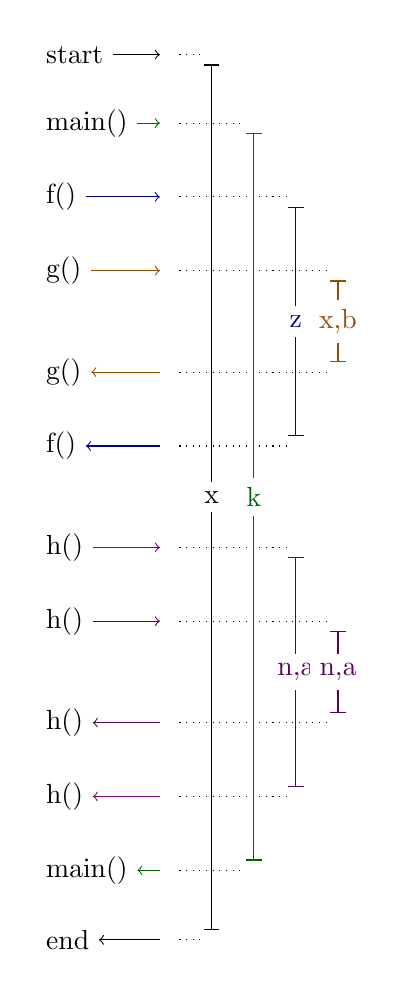
\begin{tikzpicture} 
\matrix [column sep=3mm,ampersand replacement=\&] {
\node [right](bb) {start}; \& \node (dbb) {}; \& \node (kb) {};  \\[1em]
\node [right](bm) {main()}; \& \node (dbm) {}; \&  \& \node (mb) {}; \\[1em]
\node [right](bf) {f()}; \& \node (dbf) {}; \&  \&  \& \node (fb) {}; \\[1em]
\node [right](bg) {g()}; \& \node (dbg) {}; \&  \&  \& \& \node (gb) {}; \\[2em]
\node [right](cg) {g()}; \& \node (dcg) {}; \&  \&  \& \& \node (gc) {}; \\[1em]
\node [right](cf) {f()}; \& \node (dcf) {}; \&  \&  \& \node (fc) {}; \\[2em]
\node [right](bh1) {h()}; \& \node (dbh1) {}; \&  \&  \& \node (h1b) {}; \\[1em]
\node [right](bh2) {h()}; \& \node (dbh2) {}; \&  \&  \& \& \node (h2b) {}; \\[2em]
\node [right](ch2) {h()}; \& \node (dch2) {}; \&  \&  \& \& \node (h2c) {}; \\[1em]
\node [right](ch1) {h()}; \& \node (dch1) {}; \&  \&  \& \node (h1c) {}; \\[1em]
\node [right](cm) {main()}; \& \node (dcm) {}; \&  \& \node (mc) {}; \\[1em]
\node [right](cb) {end}; \& \node (dcb) {}; \& \node (kc) {};  \\[1em]
};
\draw [->] (bb) -- (dbb);	\draw [dotted] (dbb) -- (kb);
\draw [green!40!black,->] (bm) -- (dbm);  		\draw [dotted] (dbm) -- (mb);
\draw [blue!60!black,->] (bf) -- (dbf);   		\draw [dotted] (dbf) -- (fb);
\draw [orange!60!black,->] (bg) -- (dbg);    		\draw [dotted] (dbg) -- (gb);
\draw [orange!60!black,<-] (cg) -- (dcg);  		\draw [dotted] (dcg) -- (gc);
\draw [blue!60!black,<-] (cf) -- (dcf);   		\draw [dotted] (dcf) -- (fc);
\draw [green!40!black,<-] (cm) -- (dcm);  		\draw [dotted] (dcm) -- (mc);
\draw [violet,->] (bh1) -- (dbh1);   		\draw [dotted] (dbh1) -- (h1b);
\draw [violet!70!black,->] (bh2) -- (dbh2);  		\draw [dotted] (dbh2) -- (h2b);
\draw [violet!70!black,<-] (ch2) -- (dch2);  		\draw [dotted] (dch2) -- (h2c);
\draw [violet,<-] (ch1) -- (dch1);   		\draw [dotted] (dch1) -- (h1c);
\draw [<-] (cb) -- (dcb);	\draw [dotted] (dcb) -- (kc);
\draw [|-|] (kb) -- node [fill=white] {x} (kc);
\draw [|-|,green!40!black] (mb) -- node [fill=white] {k} (mc);
\draw [|-|,blue!60!black] (fb) -- node [fill=white] {z} (fc);
\draw [|-|,orange!60!black] (gb) -- node [fill=white] {x,b} (gc);
\draw [|-|,violet!70!black] (h1b) -- node [fill=white] {n,a} (h1c);
\draw [|-|,violet!70!black] (h2b) -- node [fill=white] {n,a} (h2c);
\end{tikzpicture}

\end{multicols}
  
%%%%%%%%%%%%%%%%%%%%%%%%%%%%%%%%%%%%%%%%%%%%%%%%%%%%%%%%%%%%%%%%%%%%%

%%%%%%%%%%%%%%% Example of Heap Variables %%%%%%%%%%%%%%%

\begin{listing}[H]

\begin{minted}{c}
double *p;

int h() { ...
}

void g() { ...
  p = malloc(sizeof(double));
}

int f() { ...
  g(); ...
}

int main() { ...
  f();    ...
  h();    ...;
  free(p); ...
}
\end{minted}

\caption{Example of Heap Variables.}
\label{code:code-4}

\end{listing}

\begin{center}
  \begin{tikzpicture}
    \matrix [ampersand replacement=\&, column sep=5mm, row sep=1mm] {
    \node (bb) {start}; \& \node (bm) {main()}; \& \node (bf) {f()}; \& 
    \node (bg) {g()}; \& \node (cg) {g()}; \& \node (cf) {f()}; \& 
    \node (bh1) {h()}; \& 
    \node (ch1) {h()}; \& \node (cm) {main()}; \& \node (cb) {end}; \\[.5em]
    \node (dbb) {}; \& \node (dbm) {}; \& \node (dbf) {}; \& 
    \node (dbg) {}; \& \node (dcg) {}; \& \node (dcf) {}; \& 
    \node (dbh1) {}; \&
    \node (dch1) {}; \& \node (dcm) {}; \& \node (dcb) {}; \\[.2em]
    \node (kb) {} ;\& \& \& \& \& \& \& \& \& \node (kc) {}; \\[.2em] 
    \& \& \& \node (yb) {}; \& \& \& \&  \& \node (yc) {}; \& \\
    };
    \draw [->] (bb) -- (dbb);
    \draw [|-|] (kb) -- node [fill=white] {global: p} (kc);
    \draw [blue!90!black,|-|] (yb) +(5mm,0) -- node [fill=white] {heap variable: *p} ($(yc) - (5mm,0)$);
    \draw [green!40!black,->] (bm) -- (dbm); 
    \draw [blue!60!black,->] (bf) -- (dbf); 
    \draw [orange!60!black,->] (bg) -- (dbg);  
    \draw [orange!60!black,<-] (cg) -- (dcg);
    \draw [blue!60!black,<-] (cf) -- (dcf); 
    \draw [violet,->] (bh1) -- (dbh1); 
    \draw [violet,<-] (ch1) -- (dch1); 
    \draw [green!40!black,<-] (cm) -- (dcm);
    \draw [<-] (cb) -- (dcb);
  \end{tikzpicture}
\end{center}
  
%%%%%%%%%%%%%%%%%%%%%%%%%%%%%%%%%%%%%%%%%%%%%%%%%%%%%%%%%

\begin{multicols*}{2}
\setlength{\columnsep}{1.5cm}
\setlength{\columnseprule}{0.2pt}
